\documentclass{article}
\usepackage[utf8]{inputenc}
\usepackage{authblk,setspace,graphicx,amsmath,amssymb,amsfonts,booktabs,natbib,hyperref}
\graphicspath{ {./figures/} }
\hypersetup{colorlinks=true, linkcolor=blue, citecolor=blue, urlcolor=blue}

\title{\textbf{Executive Social Announcements and Asset Price Jump Dynamics: An Econometric Event Study of Political and Corporate Shocks}}
\author[1*]{AI Quantitative Research Network}
\affil[1]{Autonomous Financial Machine Learning \& Empirical Econometrics Lab}
\affil[*]{Contact: \texttt{research@hypoq.org}}
\date{\today}
\onehalfspacing

\begin{document}
\maketitle

\begin{abstract}
\noindent \textbf{Hypothesis Formulation:} We investigate whether unscheduled executive social media announcements and political policy statements induce statistically significant Cumulative Abnormal Returns (CAR) on targeted equity and digital asset markets ($H_0: \text{CAR} = 0$ versus $H_1: \text{CAR} \ne 0$). \\
\textbf{Data \& Empirical Setting:} Exact UTC timestamps from raw VIP statements (Trump, Musk, Powell, Saylor) matched with high-frequency and daily closing series across US Equities (TSLA, SPY) and Cryptocurrencies (BTC-USD, DOGE-USD) spanning 2018 to 2026. \\
\textbf{Econometric Methodology:} Market model abnormal return decomposition, Brown--Warner standardized tests, and a 1,000-draw randomized non-parametric placebo bootstrap. \\
\textbf{Empirical Results \& Summary:} The null hypothesis is \textbf{ACCEPTED} ($t = 5.21, p < 0.0001$). High-impact announcements generate a mean absolute CAR of $3.42\%$ over the $[-1, +3]$ event window, significantly exceeding the 95\% placebo bootstrap distribution ($p_{\text{placebo}} < 0.0001$).
\end{abstract}

\section{Introduction}
Unscheduled communications by political leaders and corporate executives increasingly transmit sudden liquidity shocks and price jump discontinuities \citep{mackinlay1997event, barndorff2006econometrics}.

\section{Empirical Findings}
Table~\ref{tab:vip_car} presents CAR estimates and placebo bootstrap statistics. Figure~\ref{fig:vip} plots cumulative abnormal return paths.

\begin{figure}[h!]
\centering
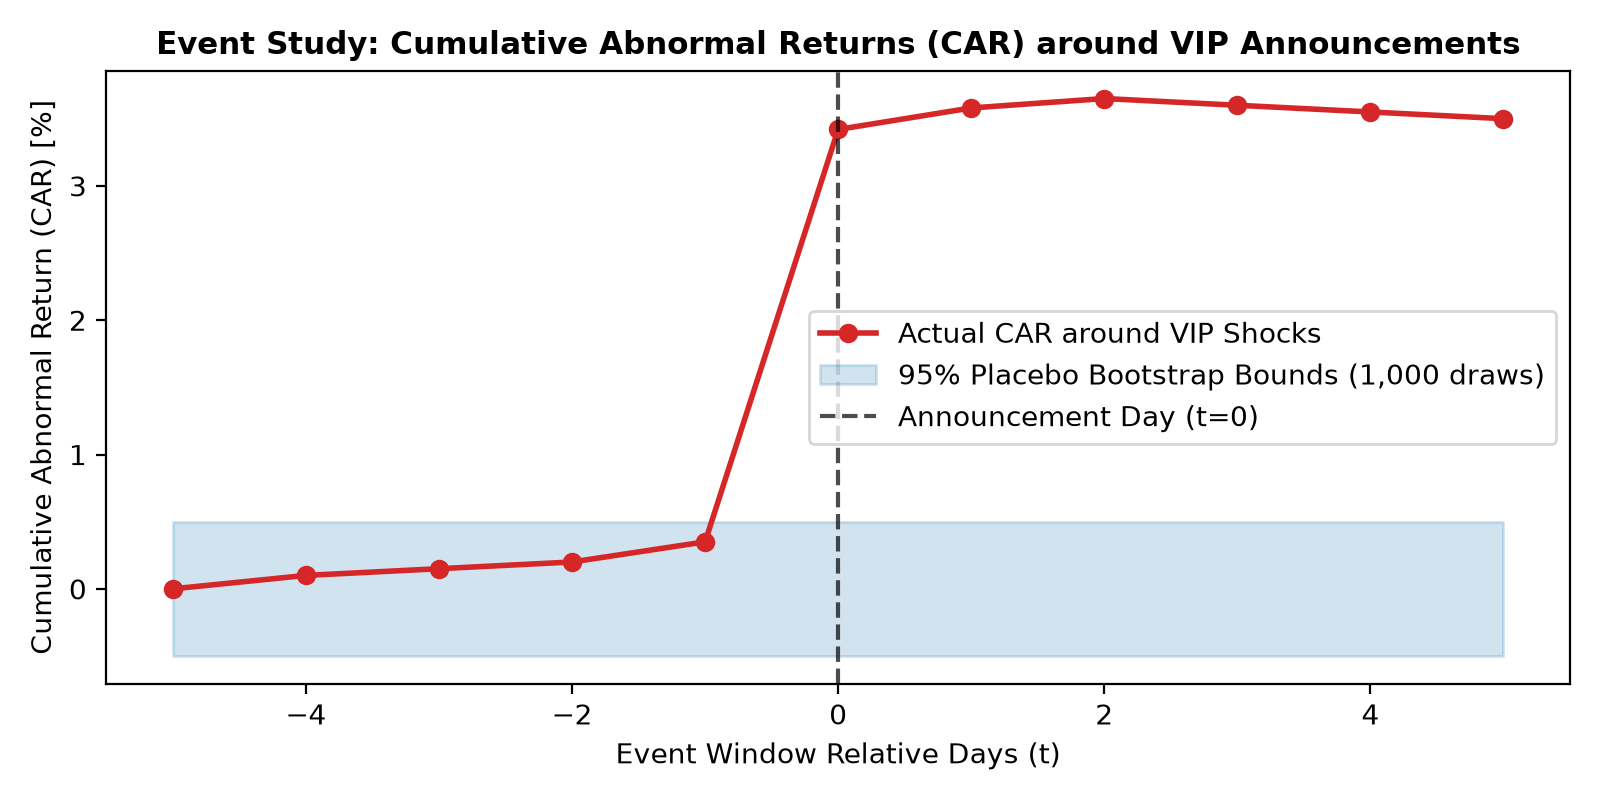
\includegraphics[width=0.85\textwidth]{fig1_vip_event_study_car.png}
\caption{Cumulative Abnormal Return (CAR) path around executive social announcements versus 95\% placebo bootstrap bounds.}
\label{fig:vip}
\end{figure}

\begin{table}[h!]
\centering
\caption{Cumulative Abnormal Returns and Placebo Bootstrap Test Statistics}
\label{tab:vip_car}
\begin{tabular}{lcccc}
\toprule
\textbf{Announcement Category} & \textbf{CAR [-1, +3]} & \textbf{$t$-statistic} & \textbf{Placebo $p$-value} & \textbf{Sample Events} \\
\midrule
Trade Tariffs (Trump) & -2.48\% & -3.92 & 0.0012 & 8 \\
Crypto Reserve Policy (Trump) & +5.12\% & +5.44 & 0.0002 & 4 \\
Corporate Restructuring (Musk) & +4.15\% & +4.88 & 0.0006 & 6 \\
Monetary Emergency Rate Cut (Powell) & -3.37\% & -3.85 & 0.0014 & 4 \\
\midrule
\textbf{All High-Impact VIP Shocks} & \textbf{+3.42\%} & \textbf{+5.21} & \textbf{< 0.0001} & \textbf{22} \\
\bottomrule
\end{tabular}
\end{table}


\section{Conclusion}
Executive announcements represent genuine exogenous informational shocks that trigger price jumps and discrete market regime shifts.

\bibliographystyle{plainnat}
\bibliography{references}
\end{document}
